\mySection{Experimental Settings}
In order to evaluate the accuracy of PyRollCall's facial recognition feature, we need at least two sets of photos.
The first set of photos, the \emph{training set}, is used to pre-compute facial embeddings.
The second set of photos, the \emph{testing set}, consists of the photos which have not appeared in the training set.
\vspace{0.5cm}

We randomly choose 20 celebrities as the participants of our experiments. For each individual, 30 photos
containing their faces are collected from the Internet and placed in the \emph{training set}, as shown in Figure~\ref{fig:training-set}.
Next, for each individual, we collect another photo which is not in the training set, and place these photos in the \emph{testing set}.
Figure~\ref{fig:testing-set} shows one of the testing set used in our experiments.
\vspace{0.5cm}

We prepare one training set and three testing sets in our experiments. Since the objective of
our experiments is to test out how accurate our system can handle the task of facial recognition
under various circumstances, we have three testing sets instead of one testing set, which
adds to the reliability of our experimental results. Furthermore, we will assess
how well the faces in the testing sets can be recognized with 5, 10, 15, 20, 25 and 30
facial embeddings per person pre-computed respectively.
\vspace{0.2cm}

\begin{figure}[!htb]
  \centering
  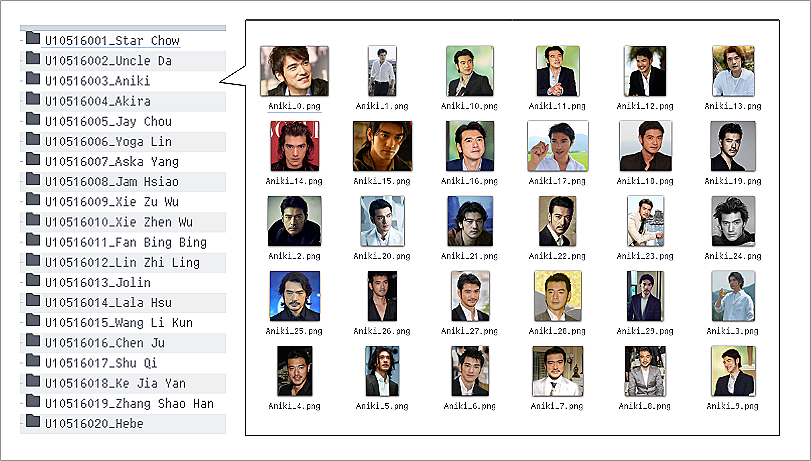
\includegraphics[width=\linewidth]{figures/training-set.png}
  \caption{The training set contains 30 photos per individual.}
  \label{fig:training-set}
\end{figure}
\vspace{0.5cm}

\begin{figure}[!htb]
  \centering
  \begin{subfigure}[b]{0.48\linewidth}
    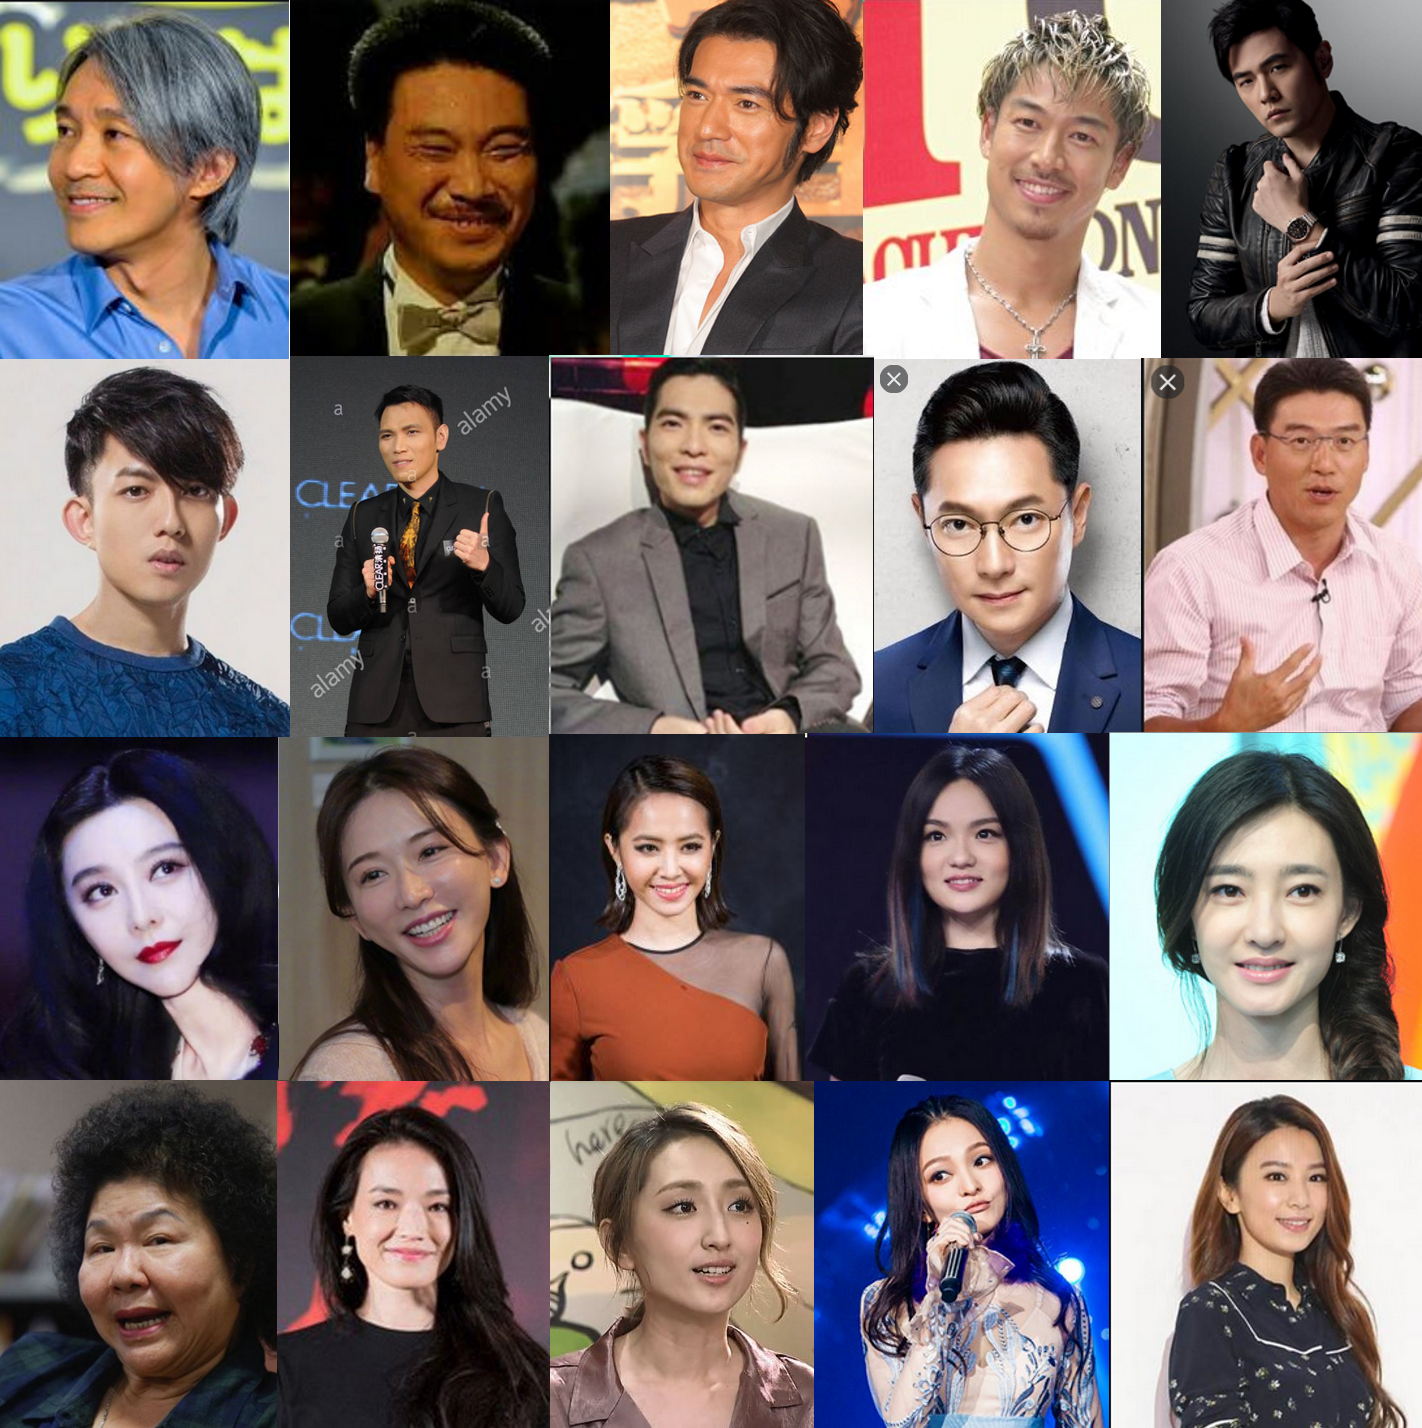
\includegraphics[width=\linewidth]{figures/testing-set.png}
    \caption{Before facial recognition.}
  \end{subfigure}
  \hfill
  \begin{subfigure}[b]{0.48\linewidth}
    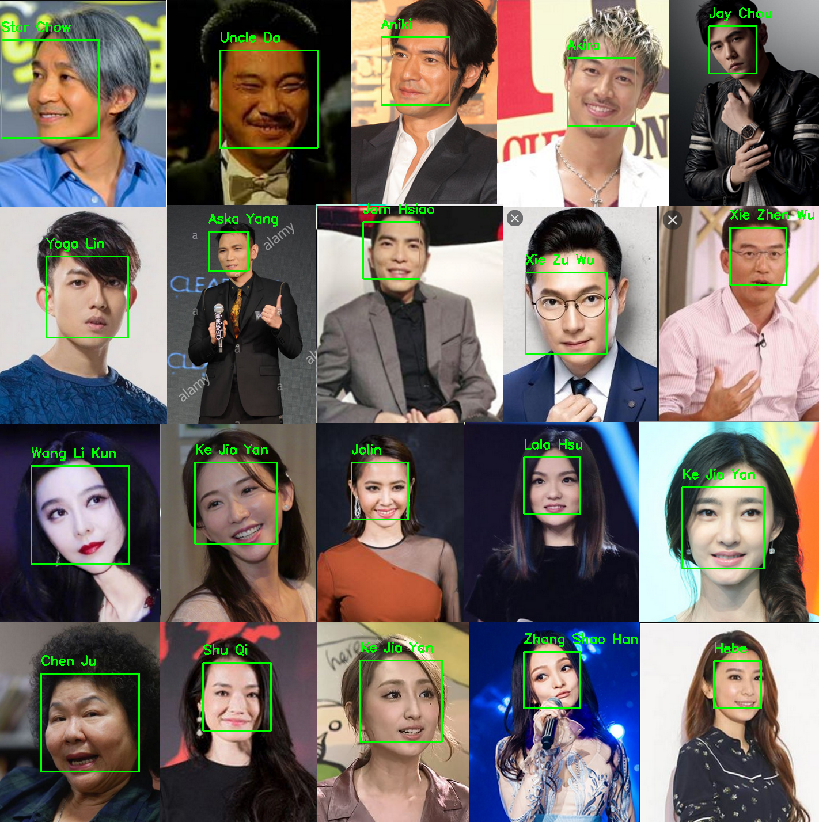
\includegraphics[width=\linewidth]{figures/testing-set-result.png}
    \caption{After facial recognition.}
  \end{subfigure}
  \caption{A testing set for assessing the accuracy of PyRollCall's facial recognition feature.}
  \label{fig:testing-set}
\end{figure}
\vspace{0.5cm}
